\chapter{Εισαγωγή}

\section{Διατύπωση του Προβλήματος}
\paragraph*{}
Για τον άνθρωπο η αντίληψη του κόσμου μέσω της όρασης είναι κάτι αρκετά εύκολο. Μπορεί να ξεχωρίσει αντικείμενα, σκηνές, πρόσωπα κτλ χωρίς να καταβάλει ιδιαίτερη προσπάθεια. Ακόμα είναι δυνατό να αναγνωρίσει συναισθήματα ή και προθέσεις μέσω των εκφράσεων του προσώπου ή τη στάση του σώματος. Για έναν υπολογιστή, όμως, κάτι αντίστοιχο είναι ένα αρκετά δύσκολο εγχείρημα.

\paragraph*{}
Ήδη από τη δεκαετία του '70 στον τομέα της μηχανικής όρασης γίνονται πολλές προσπάθειες και έχει υπάρξει μεγάλη πρόοδος, σε θέματα επεξεργασίας, αναγνώρισης και κατηγοριοποίησης εικόνων. Πολλές πτυχές αυτού του τομέα χρησιμοποιούνται σήμερα, τόσο στη βιομηχανία, όσο και σε προσωπικές συσκευές. Παρόλα αυτά ο κλάδος της μηχανικής όρασης, θεωρείται πως χρειάζεται πολλή περισσότερη ανάπτυξη, προκειμένου ένας υπολογιστής να αντιλαμβάνεται τον κόσμο μέσω της όρασης όπως ένας άνθρωπος, αν αυτό είναι δυνατό να συμβεί ολοκληρωτικά.

\paragraph*{}
Προκειμένου ένας υπολογιστής να ταξινομήσει σωστά ή να αναγνωρίσει μέρος μιας εικόνας, θα πρέπει τα δεδομένα που παρέχονται να είναι σε μορφή που ευνοεί κάτι τέτοιο. Υπάρχει, λοιπόν, η ανάγκη για αναπαράσταση των εικόνων (ή μέρος αυτών) με τρόπο που δεν επηρεάζεται από τυχόν αλλαγές στην ίδια την εικόνα, όπως είναι περιστροφή, αλλαγή κλίμακας, προσθήκη θορύβου κτλ.
\paragraph*{}
Αυτό επιχειρούν να υλοποιήσουν οι τοπικοί περιγραφείς. Ένας τοπικός περιγραφέας δημιουργεί ψηφιακή αναπαράσταση (συνήθως ένα διάνυσμα) για μια γειτονιά της εικόνας. Στόχος είναι το διάνυσμα αυτό να μένει όσο το δυνατόν ανεπηρέαστο σε αλλαγές που μπορεί να εφαρμοστούν στην εκάστοτε γειτονιά, την οποία περιγράφει. Δημιουργώντας πολλά τέτοια διανύσματα (Local Features) για γειτονιές που καλύπτουν όλη την έκταση της εικόνας, είναι δυνατό, με χρήση του μοντέλου Bag of Words, να παραχθεί αντιπροσωπευτική αναπαράσταση για ολόκληρη την εικόνα. Δημιουργείται δηλαδή, ένα νέο διάνυσμα, το οποίο λειτουργεί ως ολικός περιγραφέας. Το νέο αυτό διάνυσμα (Feature Vector) μπορεί να τροφοδοτηθεί σε κάποιον ταξινομητή, προκειμένου να γίνει σωστή κατηγοριοποίηση της εικόνας.

\paragraph*{}
Στην παρούσα διπλωματική εργασία επιχειρείται η υλοποίηση μιας αναπαράστασης εικόνας, η οποία να είναι απαλλαγμένη από την επιρροή μεταβολών λόγω περιστροφής, αλλαγής κλίμακας, μετατόπισης και προσθήκης θορύβου. Αυτή η αναπαράσταση λειτουργεί ως τοπικός περιγραφέας υφής, έτσι ώστε μέσω του μοντέλου Bag of Words να παραχθούν ολικοί περιγραφείς εικόνων. Ο τρόπος υλοποίησης του προτεινόμενου περιγραφέα αναλύεται στο Κεφάλαιο \ref{chap:sug}.


\section{Υπάρχουσες Μέθοδοι}

Για την αναπαράσταση και περιγραφή μιας εικόνας έχουν αναπτυχθεί πολλές μέθοδοι και διάφοροι αλγόριθμοι στον τομέα της τεχνητής όρασης. Παρακάτω περιγράφεται το μοντέλο Bag of Words, το οποίο χρησιμοποιείται στα πλαίσια της εργασίας για την παραγωγή των ολικών περιγραφέων, καθώς και δύο πολύ σημαντικοί τοπικοί περιγραφείς, ο SIFT και ο SURF.

\subsection{Μοντέλο Bag of Words}
\paragraph*{}
Το μοντέλο Bag of Words \cite{bow} αποτελεί μια απλοποιημένη αναπαράσταση της εικόνας. Προκειμένου να παραχθεί ο περιγραφέας της εικόνας, αυτή αντιμετωπίζεται όπως θα αντιμετωπιζόταν ένα έγγραφο κειμένου. Εξάγονται, δηλαδή οι εικονικές "λέξεις", τις οποίες περιέχει και έτσι τελικά η εικόνα χαρακτηρίζεται από το πόσες και ποιες "λέξεις" περιέχει.

\paragraph*{}
Για τη δημιουργία ολικών περιγραφέων μέσω του μοντέλου Bag of Words, αρχικά εφαρμόζεται στην εικόνα πυκνό πλέγμα σταθερού βήματος. Σε \textit{κάθε} κόμβο του πλέγματος υπολογίζεται ένας τοπικός περιγραφέας, που περιγράφει μια μικρή γειτονιά γύρω από τον κόμβο. Αυτή η διαδικασία επαναλαμβάνεται για πλήθος εικόνων και έτσι παράγεται ένα σύνολο τοπικών περιγραφέων.

\paragraph*{}
Στη συνέχεια, οι τοπικοί περιγραφείς ομαδοποιούνται σύμφωνα με το περιεχόμενό τους και κάθε ομάδα αντιπροσωπεύεται από ένα διάνυσμα μήκους όσο και τα διανύσματα των τοπικών περιγραφέων. Το σύνολο των διανυσμάτων που αντιπροσωπεύουν τις ομάδες που δημιουργήθηκαν αποτελούν το Codebook, δηλαδή το λεξικό των εικονικών λέξεων που εντοπίστηκαν στις εικόνες, από τις οποίες παράχθηκαν οι τοπικοί περιγραφείς.

\paragraph*{}
Πλέον με βάση το Codebook που έχει δημιουργηθεί, μπορεί μια εικόνα να αναπαρασταθεί σύμφωνα με αυτό. Παράγονται οι τοπικοί περιγραφείς σε κάθε κόμβο του πλέγματος που εφαρμόζεται στην εικόνα, όπως αναφέρθηκε παραπάνω και στη συνέχεια ο κάθε περιγραφέας αντιστοιχίζεται σε μια ομάδα/εικονική λέξη, ανάλογα με την απόστασή του από το αντίστοιχο διάνυσμα που την αντιπροσωπεύει. Τελικά δημιουργείται ένα ιστόγραμμα που απεικονίζει τη συχνότητα εμφάνισης της κάθε λέξης του Codebook στην εικόνα.

\paragraph*{}
Το ιστόγραμμα που παράγεται αποτελεί τον ολικό περιγραφέα της εικόνας. Πρόκειται, δηλαδή για ένα διάνυσμα, το οποίο έχει τόσα στοιχεία, όσες και οι εικονικές λέξεις του Codebook, όπου το κάθε στοιχείο μας δίνει τη συχνότητα εμφάνισης της αντίστοιχης λέξης. Στο τέλος, το διάνυσμα που προκύπτει για την κάθε εικόνα κανονικοποιείται ώστε τα στοιχεία του να αθροίζουν σε σταθερό αριθμό (συνήθως μονάδα).


\subsection{SIFT} \label{subsec:sift}
\paragraph*{}
Ο αλγόριθμος SIFT \cite{sift} (Scale Invariant Feature Transform) παράγει τοπικούς περιγραφείς, οι οποίοι είναι ανεξάρτητοι από την κλιμάκωση και τον προσανατολισμό της εικόνας.
\paragraph*{}
Προκειμένου να υπάρχει ανεξαρτησία από τον προσανατολισμό της εικόνας, αρχικά υπολογίζονται τα παρακάτω δύο μεγέθη σε κάθε σημείο:

\begin{equation}
m(x,y) = \sqrt{(I(x+1,y) - I(x-1,y))^2 + (I(x,y+1) - I(x,y-1))^2}
\end{equation}

\begin{equation}
\theta(x,y) = \tan^{-1}((I(x,y+1)-I(x,y-1))/(I(x+1,y)-I(x-1,y))),
\end{equation}
όπου $I(x,y)$ η εικόνα εισόδου, $m(x,y)$ το μέγεθος (gradient magnitude) και $\theta(x,y)$ ο προσανατολισμός (gra\-dient orientation) της κλίσης. Στη συνέχεια εφαρμόζεται η γκαουσιανή συνάρτηση με $\sigma$ ίσο με το μισό του πλάτους της εικόνας, έτσι ώστε όσο μεγαλώνει η απόσταση από το κέντρο, οι αντίστοιχες κλίσεις να έχουν μικρότερη βαρύτητα. Έπειτα, δημιουργούνται ιστογράμματα προσανατολισμού σε υποπεριοχές της εικόνας λαμβάνοντας υπόψιν όλα τα $m(x,y)$ και $\theta(x,y)$ που υπολογίσθηκαν. Οι κορυφές αυτών των ιστογραμμάτων αντιστοιχούν στις εντονότερες κατευθύνσεις των τοπικών κλίσεων και αυτές καθορίζουν τον προσανατολισμό της κάθε υποπεριοχής. Τελικά το διάνυσμα του περιγραφέα περιέχει τους εντονότερους προσανατολισμούς των περιοχών. Το διάνυσμα αυτό κανονικοποιείται, ώστε να έχει μέτρο μονάδα. Έπειτα γίνεται έλεγχος στα στοιχεία του, στα οποία εφαρμόζεται ένα ανώφλι 0.2 και, πλέον στο νέο διάνυσμα, γίνεται ξανά κανονικοποίηση του μέτρου στη μονάδα. Αυτές οι ενέργειες οδηγούν στην ανεξαρτησία σε αλλαγές της φωτεινότητας.

\paragraph*{}
Όσον αφορά στην ανεξαρτησία από την κλιμάκωση, υπάρχει η δυνατότητα, μετά από επιλογή της κατάλληλης κλίμακας (ή κλιμάκων), να δημιουργηθούν αντίγραφα της εικόνας, τα οποία κλιμακώνονται με χρήση γκαουσιανού φίλτρου. Πλέον η διαδικασία που περιγράφηκε παραπάνω, επαναλαμβάνεται σε κάθε εκδοχή της εικόνας που έχει παραχθεί.


%Η διαδικασία παραγωγής των περιγραφέων της εικόνας χωρίζεται σε τέσσερα στάδια \cite{sift}, όπου σε κάθε ένα από αυτά, εφαρμόζονται φίλτρα και έλεγχοι στην εικόνα, έτσι ώστε ο τοπικός περιγραφέας που θα παραχθεί να περιέχει την πιο χρήσιμη πληροφορία. Τα τέσσερα στάδια είναι τα παρακάτω:

%\begin{enumerate}[i]
%  \item Εύρεση ακρότατων ως προς το χώρο και την κλιμάκωση (Scale-space extrema detection)
%  \item Ανίχνευση σημείων ενδιαφέροντος (Keypoint localization)
%  \item Ανάθεση προσανατολισμού (Orientation assignment)
%  \item Δημιουργία του περιγραφέα του σημείου ενδιαφέροντος (Keypoint descriptor)
%\end{enumerate}

%\paragraph*{Εύρεση ακρότατων ως προς το χώρο και την κλιμάκωση}
%Αρχικά ο αλγόριθμος, εφαρμόζοντας στην εικόνα διαδοχικά φίλτρα εντοπίζει υποψήφια σημεία ακρότατων (μετέπειτα υποψήφια σημεία ενδιαφέροντος), τα οποία στη συνέχεια ελέγχονται για να εξακριβωθεί αν όντως είναι ελάχιστα ή μέγιστα. Προκειμένου τα ακρότατα να είναι ελάχιστα ή μέγιστα, όχι μόνο στο χώρο, αλλά και στην κλιμάκωση, εφαρμόζεται επανειλημμένα στην εικόνα η γκαουσιανή συνάρτηση:
%
%\begin{equation}
%G(x,y,\sigma) = \dfrac{1}{2\pi\sigma^2} e^{-\frac{x^2 + y^2}{2\sigma^2}}
%\end{equation}
%δημιουργώντας, έτσι, εκδοχές της ίδιας εικόνας, σε διαφορετική κλίμακα. Αν θεωρήσουμε $I(x,y)$ μία εικόνα και $G(x,y,\sigma)$  την γκαουσιανή συνάρτηση, τότε οι νέες εικόνες που προκύπτουν, $L(x,y,\sigma)$, είναι το αποτέλεσμα της συνέλιξης της εικόνας με την γκαουσιανή συνάρτηση:
%
%\begin{equation}
%L(x,y,\sigma)=G(x,y,\sigma)*I(x,y)
%\end{equation}
%Επιπλέον, αφού δημιουργηθεί μια παρτίδα από $L(x,y,\sigma)$, τότε η αρχική εικόνα υπόκειται σε υποδιπλασιασμό των διαστάσεών της και σε αυτή τη νέα εικόνα εφαρμόζεται ξανά η γκαουσιανή συνάρτηση. Με αυτό τον τρόπο δημιουργούνται πολλές παρτίδες από $L(x,y,\sigma)$ με ίδια $\sigma$, αλλά διαφορετικών διαστάσεων.

%\paragraph*{}
%Στη συνέχεια υπολογίζεται η συνάρτηση διαφοράς των εικόνων διαφορετικής κλιμάκωσης (difference-of-Gaussian function) $D(x,y,\sigma)$:
%
%\begin{align}
%D(x,y,\sigma) &= (G(x,y,k\sigma)-G(x,y,\sigma))*I(x,y) \\
%&= L(x,y,k\sigma) - L(x,y,\sigma) \nonumber
%\end{align}
%Ουσιαστικά, για τον υπολογισμό της $D(x,y,\sigma)$ αφαιρούνται εικόνες, των οποίων η κλίμακα διαφέρει κατά ένα σταθερό πολλαπλασιαστικό παράγοντα $k$. Στο Σχήμα \ref{fig:dog} φαίνεται η διαδικασία υπολογισμού της $D(x,y,\sigma)$.
%
%\begin{figure}[t]
%        \centering
%                \centerline{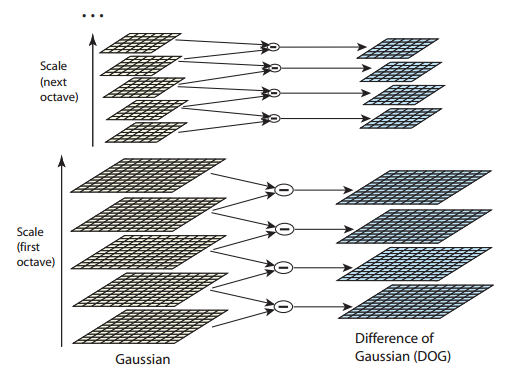
\includegraphics[scale = 0.8]{./images/d-o-g.png}}
%                \caption{Υπολογισμός της $D(x,y,\sigma)$}
%                \label{fig:dog}
%\end{figure}
%
%\paragraph*{}
%Μετά τον υπολογισμό των $D(x,y,\sigma)$, το κάθε στοιχείο τους συγκρίνεται με τα οκτώ γειτονικά του, καθώς επίσης και με τα εννιά γειτονικά του σημεία από τα επίπεδα πάνω και κάτω από το ίδιο (των εικόνων που ανήκουν στην ίδια παρτίδα). Συγκρίνεται δηλαδή, με οκτώ σημεία ίδιας κλιμάκωσης, εννιά σημεία μικρότερης και εννιά σημεία μεγαλύτερης κλιμάκωσης. Το εκάστοτε σημείο επιλέγεται ως μέγιστο (ελάχιστο) στην περίπτωση που είναι μεγαλύτερο (μικρότερο) από \textit{όλα} τα γειτονικά του (Σχ. \ref{fig:extrema}).
%
%\begin{figure}
%        \centering
%                \centerline{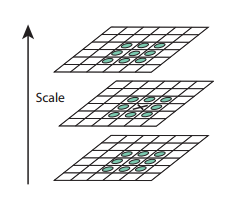
\includegraphics[scale = 0.8]{./images/findExtrema.png}}
%                \caption{Σύγκριση του σημείου με τα γειτονικά του}
%                \label{fig:extrema}
%\end{figure}

%\paragraph*{Ανίχνευση σημείων ενδιαφέροντος}
%Στη συνέχεια, για κάθε υποψήφιο σημείο ενδιαφέροντος (σημεία που επιλέχθηκαν μετά από σύγκριση με τους 26 γείτονές τους) $(x,y,\sigma)$, εκφράζεται η $D(x,y,\sigma)$ μέσω του αναπτύγματος Taylor:
%
%\begin{equation}
%D(\boldsymbol{x}) = D + \frac{\partial D^T}{\partial \boldsymbol{x}} \boldsymbol{x} + \frac{1}{2} \boldsymbol{x^T} \frac{\partial^2 D}{\partial \boldsymbol{x} ^ 2} \boldsymbol{x},
%\end{equation}
%όπου $\boldsymbol{x} = [x,y,\sigma]^T$ είναι η απόσταση από το υποψήφιο σημείο ενδιαφέροντος. Η θέση του ακρότατου $\hat{\boldsymbol{x}}$  υπολογίζεται μηδενίζοντας την παράγωγο ως προς $\boldsymbol{x}$ της $D(\boldsymbol{x})$. Αν η απόσταση του ακρότατου είναι μεγαλύτερη από 0.5 ως προς οποιαδήποτε διάσταση, τότε αυτό σημαίνει πως το ακρότατο είναι πιο κοντά σε κάποιο άλλο σημείο ενδιαφέροντος. Σε αυτή την περίπτωση το υποψήφιο σημείο αλλάζει και η διαδικασία επαναλαμβάνεται για το νέο υποψήφιο σημείο ενδιαφέροντος. Η τελική απόσταση $\hat{\boldsymbol{x}}$ που υπολογίζεται προστίθεται στο υποψήφιο σημείο ενδιαφέροντος για να βρούμε τη θέση του ακρότατου.
%
%\paragraph*{}
%Μέσω της $D(\boldsymbol{x})$ είναι δυνατό να απορριφθούν ασταθή ακρότατα με χαμηλή αντίθεση (έχουν μεγάλη ευαισθησία ως προς το θόρυβο). 

%\paragraph*{Ανάθεση προσανατολισμού}
%Προκειμένου να υπάρχει ανεξαρτησία από τον προσανατολισμό της εικόνας, ανατίθεται σε κάθε σημείο ενδιαφέροντος προσανατολισμός, που προκύπτει από τη γειτονιά του σημείου. Με βάση την κλίμακα του σημείου επιλέγεται η $L(x,y,\sigma)$ με την πιο κοντινή κλίμακα σε αυτό. Αυτό γίνεται, ώστε να ανεξαρτητοποιηθούν οι υπολογισμοί από την κλιμάκωση. Για κάθε $L(x,y)$ αυτής της κλίμακας υπολογίζονται τα παρακάτω δύο μεγέθη:
%
%\begin{equation}
%m(x,y) = \sqrt{(L(x+1,y) - L(x-1,y))^2 + (L(x,y+1) - L(x,y-1))^2}
%\end{equation}
%
%\begin{equation}
%\theta(x,y) = \tan^{-1}((L(x,y+1)-L(x,y-1))/(L(x+1,y)-L(x-1,y))),
%\end{equation}
%όπου $m(x,y)$ το μέγεθος (gradient magnitude) και $\theta(x,y)$ ο προσανατολισμός (gra\-dient orientation) της κλίσης. Στη συνέχεια δημιουργείται ένα ιστόγραμμα του προσανατολισμού της γειτονιάς του σημείου ενδιαφέροντος, λαμβάνοντας υπόψιν το $m(x,y)$ και $\theta(x,y)$ του κάθε σημείου της γειτονιάς. Οι κορυφές αυτού του ιστογράμματος αντιστοιχούν στις εντονότερες κατευθύνσεις των τοπικών κλίσεων. Τελικά επιλέγεται η υψηλότερη κορυφή του ιστογράμματος, η οποία καθορίζει τον προσανατολισμό του σημείου. Επιπλέον επιλέγονται και όσες κορυφές είναι στο 80\%  της υψηλότερης, έτσι ώστε για περιοχές με έντονο προσανατολισμό να δημιουργηθούν πολλαπλά σημεία ενδιαφέροντος, καθένα με το δικό του προσανατολισμό.
%
%
%\paragraph*{Δημιουργία του περιγραφέα του σημείου ενδιαφέροντος}
%Στο τελικό στάδιο, για τη δημιουργία του περιγραφέα, λαμβάνονται υπόψιν τα χαρακτηριστικά που δόθηκαν στα σημεία ενδιαφέροντος σε όλα τα προηγούμενα βήματα. 
%\paragraph*{}
%Αρχικά  υπολογίζονται το μέγεθος και ο προσανατολισμός της κλίσης των περιοχών γύρω από το σημείο ενδιαφέροντος, χρησιμοποιώντας την κλίμακα που έχει ανατεθεί στο σημείο αυτό. Στη συνέχεια εφαρμόζεται γκαουσιανή συνάρτηση σε αυτή την περιοχή με $\sigma$ ίσο με το μισό του πλάτους της περιοχής, έτσι ώστε όσο μεγαλώνει η απόσταση από το σημείο ενδιαφέροντος, οι αντίστοιχες κλίσεις να έχουν μικρότερη βαρύτητα.
%\paragraph*{}
%Τέλος, δημιουργούνται ιστογράμματα προσανατολισμού σε υποπεριοχές της γειτονιάς του σημείου ενδιαφέροντος και το διάνυσμα του περιγραφέα περιέχει τους εντονότερους προσανατολισμούς αυτών των υποπεριοχών, δηλαδή τις υψηλότερες κορυφές των ιστογραμμάτων. Το διάνυσμα αυτό κανονικοποιείται, ώστε να έχει μέτρο μονάδα. Έπειτα γίνεται έλεγχος στα στοιχεία του, στα οποία εφαρμόζεται ένα ανώφλι 0.2 και, πλέον στο νέο διάνυσμα, γίνεται ξανά κανονικοποίηση του μέτρου στη μονάδα. Αυτές οι ενέργειες οδηγούν στην ανεξαρτησία σε αλλαγές της φωτεινότητας.


% ======================================================================================================================================
% ======================================================================================================================================

\subsection{SURF}
\paragraph*{}
Ο αλγόριθμος SURF \cite{surf} (Speeded-Up Robust Features), σε αντίθεση με τον SIFT υπολογίζει τον περιγραφέα χρησιμοποιώντας την ολοκληρωτική μορφή της εικόνας (integral image), και όχι αυτούσια την εικόνα. Πρόκειται για έναν πίνακα ίδιας διάστασης με την εικόνα, όπου το $(i,j)$ στοιχείο του είναι το άθροισμα του $(i,j)$ pixel της εικόνας και όλων των pixels που βρίσκονται πάνω και αριστερά από αυτό. Ο τύπος υπολογισμού δίνεται παρακάτω:

\begin{equation}
I_\Sigma(x,y) = \sum_{i=0}^{x}\sum_{j=0}^{y}I(i,j),
\end{equation}
όπου $I$ είναι η αρχική εικόνα και $I_\Sigma$ η ολοκληρωτική μορφή της. Το ενδιαφέρον με αυτή τη μορφή είναι, πως για να υπολογίσει κανείς την ολοκληρωτική μορφή μιας ορθογώνιας περιοχής της εικόνας, ανεξαρτήτου μεγέθους και θέσης, το μόνο που χρειάζεται είναι οι τιμές τεσσάρων pixel. Ένα παράδειγμα φαίνεται στην εικόνα του Σχήματος \ref{fig:integral}, όπου η ολοκληρωτική μορφή της γκρι περιοχής προκύπτει $\Sigma = I_\Sigma(A)+I_\Sigma(D)-I_\Sigma(C)-I_\Sigma(B)$. Αυτή την ιδιότητα εκμεταλλεύεται ο αλγόριθμος SURF για ελάττωση της ταχύτητας των υπολογισμών.

\begin{figure}
        \centering
                \centerline{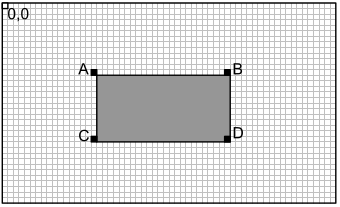
\includegraphics[scale = 1]{./images/integral.png}}
                \caption{Υπολογισμός ολοκληρωτικής μορφής}
                \label{fig:integral}
\end{figure}


\paragraph*{}
Για ανεξαρτησία από την περιστροφή ανατίθεται στην εικόνα μία "υπερισχύουσα κατεύθυνση" (dominant direction). Στη συνέχεια η εικόνα περιστρέφεται, προκειμένου να αποκτήσει τον προσανατολισμό της υπερισχύουσας κατεύθυνσης που της έχει ανατεθεί. Έπειτα χωρίζεται σε υποπεριοχές, όπου σε κάθε μία εφαρμόζεται φίλτρο Haar. Στα αποτελέσματα του φίλτρου εφαρμόζεται η γκαουσιανή συνάρτηση και αθροίζονται για την κάθε υποπεριοχή σε ένα διάνυσμα. Βάζοντας αυτά τα διανύσματα στη σειρά προκύπτει ο περιγραφέας. Τέλος, γίνεται κανονικοποίηση του μέτρου του διανύσματος στη μονάδα.


%\paragraph*{}
%Ο αλγόριθμος SURF \cite{surf} (Speeded-Up Robust Features), ανιχνεύει σημεία ενδιαφέροντος σε μια εικόνας και δημιουργεί για αυτά έναν τοπικό περιγραφέα. Οι δύο αλγόριθμοι ακολουθούν παρόμοια δομή για τη δημιουργία του περιγραφέα, παρόλα αυτά έχουν έντονες διαφορές στον τρόπο με τον οποίο υλοποιούν το κάθε βήμα.
%
%\paragraph*{}
%Κατ' αρχάς, ο SURF, υπολογίζει τον περιγραφέα χρησιμοποιώντας την ολοκληρωτική μορφή της εικόνας (integral image), και όχι αυτούσια την εικόνα. Πρόκειται για έναν πίνακα ίδιας διάστασης με την εικόνα, όπου το $(i,j)$ στοιχείο του είναι το άθροισμα του $(i,j)$ pixel της εικόνας και όλων των pixels που βρίσκονται πάνω και αριστερά από αυτό. Ο τύπος υπολογισμού δίνεται παρακάτω:
%
%\begin{equation}
%I_\Sigma(x,y) = \sum_{i=0}^{x}\sum_{j=0}^{y}I(i,j),
%\end{equation}
%όπου $I$ είναι η αρχική εικόνα και $I_\Sigma$ η ολοκληρωτική μορφή της. Το ενδιαφέρον με αυτή τη μορφή είναι, πως για να υπολογίσει κανείς την ολοκληρωτική μορφή μιας ορθογώνιας περιοχής της εικόνας, ανεξαρτήτου μεγέθους και θέσης, το μόνο που χρειάζεται είναι οι τιμές τεσσάρων pixel. Ένα παράδειγμα φαίνεται στην εικόνα του Σχήματος \ref{fig:integral}, όπου η ολοκληρωτική μορφή της γκρι περιοχής προκύπτει $\Sigma = I_\Sigma(A)+I_\Sigma(D)-I_\Sigma(C)-I_\Sigma(B)$. Αυτή την ιδιότητα εκμεταλλεύεται ο αλγόριθμος SURF για ελάττωση της ταχύτητας των υπολογισμών.
%
%\begin{figure}
%        \centering
%                \centerline{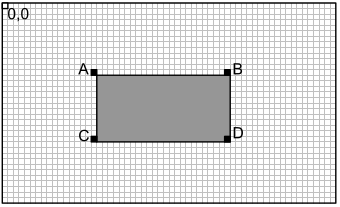
\includegraphics[scale = 1]{./images/integral.png}}
%                \caption{Υπολογισμός ολοκληρωτικής μορφής}
%                \label{fig:integral}
%\end{figure}
%
%\paragraph*{}
%Προκειμένου να εντοπιστούν τα σημεία ενδιαφέροντος της εικόνας, χρησιμοποιείται η ορίζουσα του Εσσιανού πίνακα που υπολογίζεται για το κάθε σημείο της εικόνας. Επιπλέον, για να υπάρχει ανεξαρτησία από την κλιμάκωση, όπως και στο SIFT, δημιουργούνται αντίγραφα της εικόνας σε διάφορες κλίμακες και δειγματοληψίες. Στη συνέχεια εντοπίζονται τοπικά μέγιστα με σύγκριση του κάθε στοιχείου του Εσσιανού πίνακα με τα 26 γειτονικά του. Η ακριβής θέση του ακρότατου υπολογίζεται με τον ίδιο ακριβώς τρόπο που περιγράφηκε στο Κεφ. \ref{subsec:sift}. 
%
%\paragraph*{}
%Για ανεξαρτησία από την περιστροφή ανατίθεται σε κάθε σημείο ενδιαφέροντος μία "υπερισχύουσα κατεύθυνση" (dominant direction). Στη συνέχεια ορίζεται μια γειτονιά του σημείου ενδιαφέροντος, από την οποία παράγεται ο περιγραφέας. Η γειτονιά αυτή, αρχικά περιστρέφεται, προκειμένου να αποκτήσει τον προσανατολισμό της υπερισχύουσας κατεύθυνσης που έχει ανατεθεί στο σημείο ενδιαφέροντος. Έπειτα η γειτονιά χωρίζεται σε υποπεριοχές, όπου σε κάθε μία εφαρμόζεται φίλτρο Haar. Στα αποτελέσματα του φίλτρου εφαρμόζεται η γκαουσιανή συνάρτηση και αθροίζονται για την κάθε υποπεριοχή σε ένα διάνυσμα. Βάζοντας αυτά τα διανύσματα στη σειρά προκύπτει ο περιγραφέας. Τέλος, γίνεται κανονικοποίηση του μέτρου του διανύσματος στη μονάδα.
